\documentclass{standalone}
\usepackage{tikz}
\usetikzlibrary{patterns, positioning}


\begin{document}
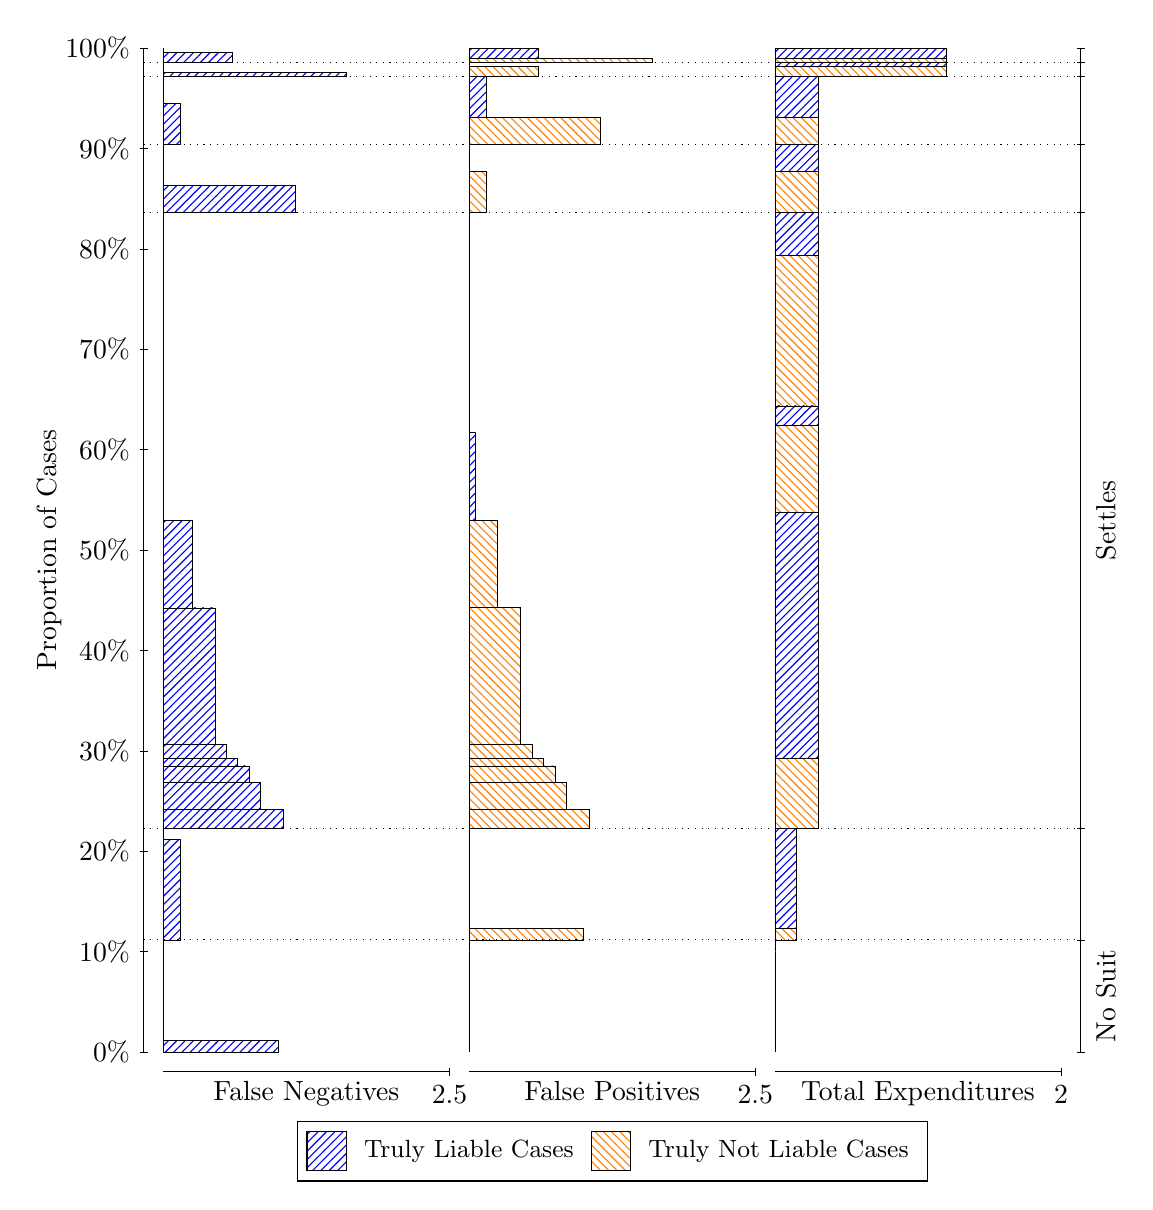
\begin{tikzpicture}
\draw[black, very thin] (1.5,1.75) -- (1.5,14.5);
\node[rotate=90, text=black, anchor=center] at (0.3, 8.125) {Proportion of Cases};
\draw[black, very thin] (1.45,1.75) -- (1.55,1.75);
\node[text=black, anchor=east] at (1.45, 1.75) {0\%};
\draw[black, very thin] (1.45,3.025) -- (1.55,3.025);
\node[text=black, anchor=east] at (1.45, 3.025) {10\%};
\draw[black, very thin] (1.45,4.3) -- (1.55,4.3);
\node[text=black, anchor=east] at (1.45, 4.3) {20\%};
\draw[black, very thin] (1.45,5.575) -- (1.55,5.575);
\node[text=black, anchor=east] at (1.45, 5.575) {30\%};
\draw[black, very thin] (1.45,6.85) -- (1.55,6.85);
\node[text=black, anchor=east] at (1.45, 6.85) {40\%};
\draw[black, very thin] (1.45,8.125) -- (1.55,8.125);
\node[text=black, anchor=east] at (1.45, 8.125) {50\%};
\draw[black, very thin] (1.45,9.4) -- (1.55,9.4);
\node[text=black, anchor=east] at (1.45, 9.4) {60\%};
\draw[black, very thin] (1.45,10.675) -- (1.55,10.675);
\node[text=black, anchor=east] at (1.45, 10.675) {70\%};
\draw[black, very thin] (1.45,11.95) -- (1.55,11.95);
\node[text=black, anchor=east] at (1.45, 11.95) {80\%};
\draw[black, very thin] (1.45,13.225) -- (1.55,13.225);
\node[text=black, anchor=east] at (1.45, 13.225) {90\%};
\draw[black, very thin] (1.45,14.5) -- (1.55,14.5);
\node[text=black, anchor=east] at (1.45, 14.5) {100\%};

\draw[black, very thin] (13.4,1.75) -- (13.4,14.5);
\draw[black, very thin] (13.35,1.75) -- (13.45,1.75);
\node[anchor=west] at (13.35, 1.75) {};
\draw[black, very thin] (13.35,3.1734) -- (13.45,3.1734);
\node[anchor=west] at (13.35, 3.1734) {};
\draw[black, very thin] (13.35,4.5933) -- (13.45,4.5933);
\node[anchor=west] at (13.35, 4.5933) {};
\draw[black, very thin] (13.35,12.415) -- (13.45,12.415);
\node[anchor=west] at (13.35, 12.415) {};
\draw[black, very thin] (13.35,13.279) -- (13.45,13.279);
\node[anchor=west] at (13.35, 13.279) {};
\draw[black, very thin] (13.35,14.143) -- (13.45,14.143);
\node[anchor=west] at (13.35, 14.143) {};
\draw[black, very thin] (13.35,14.321) -- (13.45,14.321);
\node[anchor=west] at (13.35, 14.321) {};
\draw[black, very thin] (13.35,14.5) -- (13.45,14.5);
\node[anchor=west] at (13.35, 14.5) {};

\draw[black, very thin, pattern color=blue, pattern=north east lines] (1.75,1.75) rectangle (3.2033,1.8998);
\draw[black, very thin, pattern color=orange, pattern=north west lines] (1.75,1.8998) rectangle (1.75,3.1734);
\draw[black, very thin, pattern color=blue, pattern=north east lines] (1.75,3.1734) rectangle (1.968,4.4453);
\draw[black, very thin, pattern color=orange, pattern=north west lines] (1.75,4.4453) rectangle (1.75,4.5933);
\draw[black, very thin, pattern color=blue, pattern=north east lines] (1.75,4.5933) rectangle (3.276,4.8356);
\draw[black, very thin, pattern color=blue, pattern=north east lines] (1.75,4.8356) rectangle (2.9853,5.1745);
\draw[black, very thin, pattern color=blue, pattern=north east lines] (1.75,5.1745) rectangle (2.84,5.3845);
\draw[black, very thin, pattern color=blue, pattern=north east lines] (1.75,5.3845) rectangle (2.6947,5.481);
\draw[black, very thin, pattern color=blue, pattern=north east lines] (1.75,5.481) rectangle (2.5493,5.6577);
\draw[black, very thin, pattern color=blue, pattern=north east lines] (1.75,5.6577) rectangle (2.404,7.3912);
\draw[black, very thin, pattern color=blue, pattern=north east lines] (1.75,7.3912) rectangle (2.1133,8.5042);
\draw[black, very thin, pattern color=orange, pattern=north west lines] (1.75,8.5042) rectangle (1.75,12.415);
\draw[black, very thin, pattern color=blue, pattern=north east lines] (1.75,12.415) rectangle (3.4213,12.757);
\draw[black, very thin, pattern color=orange, pattern=north west lines] (1.75,12.757) rectangle (1.75,13.279);
\draw[black, very thin, pattern color=blue, pattern=north east lines] (1.75,13.279) rectangle (1.968,13.801);
\draw[black, very thin, pattern color=orange, pattern=north west lines] (1.75,13.801) rectangle (1.75,14.143);
\draw[black, very thin, pattern color=blue, pattern=north east lines] (1.75,14.143) rectangle (4.0753,14.194);
\draw[black, very thin, pattern color=orange, pattern=north west lines] (1.75,14.194) rectangle (1.75,14.321);
\draw[black, very thin, pattern color=blue, pattern=north east lines] (1.75,14.321) rectangle (2.622,14.449);
\draw[black, very thin, pattern color=orange, pattern=north west lines] (1.75,14.449) rectangle (1.75,14.5);
\draw[black, very thin, pattern color=orange, pattern=north west lines] (5.6333,1.75) rectangle (5.6333,3.0237);
\draw[black, very thin, pattern color=blue, pattern=north east lines] (5.6333,3.0237) rectangle (5.6333,3.1734);
\draw[black, very thin, pattern color=orange, pattern=north west lines] (5.6333,3.1734) rectangle (7.0867,3.3215);
\draw[black, very thin, pattern color=blue, pattern=north east lines] (5.6333,3.3215) rectangle (5.6333,4.5933);
\draw[black, very thin, pattern color=orange, pattern=north west lines] (5.6333,4.5933) rectangle (7.1593,4.8356);
\draw[black, very thin, pattern color=orange, pattern=north west lines] (5.6333,4.8356) rectangle (6.8687,5.1744);
\draw[black, very thin, pattern color=orange, pattern=north west lines] (5.6333,5.1744) rectangle (6.7233,5.3843);
\draw[black, very thin, pattern color=orange, pattern=north west lines] (5.6333,5.3843) rectangle (6.578,5.4809);
\draw[black, very thin, pattern color=orange, pattern=north west lines] (5.6333,5.4809) rectangle (6.4327,5.6575);
\draw[black, very thin, pattern color=orange, pattern=north west lines] (5.6333,5.6575) rectangle (6.2873,7.3913);
\draw[black, very thin, pattern color=orange, pattern=north west lines] (5.6333,7.3913) rectangle (5.9967,8.5043);
\draw[black, very thin, pattern color=blue, pattern=north east lines] (5.6333,8.5043) rectangle (5.706,9.6172);
\draw[black, very thin, pattern color=blue, pattern=north east lines] (5.6333,9.6172) rectangle (5.6333,12.415);
\draw[black, very thin, pattern color=orange, pattern=north west lines] (5.6333,12.415) rectangle (5.8513,12.937);
\draw[black, very thin, pattern color=blue, pattern=north east lines] (5.6333,12.937) rectangle (5.6333,13.279);
\draw[black, very thin, pattern color=orange, pattern=north west lines] (5.6333,13.279) rectangle (7.3047,13.621);
\draw[black, very thin, pattern color=blue, pattern=north east lines] (5.6333,13.621) rectangle (5.8513,14.143);
\draw[black, very thin, pattern color=orange, pattern=north west lines] (5.6333,14.143) rectangle (6.5053,14.27);
\draw[black, very thin, pattern color=blue, pattern=north east lines] (5.6333,14.27) rectangle (5.6333,14.321);
\draw[black, very thin, pattern color=orange, pattern=north west lines] (5.6333,14.321) rectangle (7.9587,14.373);
\draw[black, very thin, pattern color=blue, pattern=north east lines] (5.6333,14.373) rectangle (6.5053,14.5);
\draw[black, very thin, pattern color=orange, pattern=north west lines] (9.5167,1.75) rectangle (9.5167,3.0237);
\draw[black, very thin, pattern color=blue, pattern=north east lines] (9.5167,3.0237) rectangle (9.5167,3.1734);
\draw[black, very thin, pattern color=orange, pattern=north west lines] (9.5167,3.1734) rectangle (9.7892,3.3215);
\draw[black, very thin, pattern color=blue, pattern=north east lines] (9.5167,3.3215) rectangle (9.7892,4.5933);
\draw[black, very thin, pattern color=orange, pattern=north west lines] (9.5167,4.5933) rectangle (10.062,5.4809);
\draw[black, very thin, pattern color=blue, pattern=north east lines] (9.5167,5.4809) rectangle (10.062,8.6006);
\draw[black, very thin, pattern color=orange, pattern=north west lines] (9.5167,8.6006) rectangle (10.062,9.7136);
\draw[black, very thin, pattern color=blue, pattern=north east lines] (9.5167,9.7136) rectangle (10.062,9.9559);
\draw[black, very thin, pattern color=orange, pattern=north west lines] (9.5167,9.9559) rectangle (10.062,11.866);
\draw[black, very thin, pattern color=blue, pattern=north east lines] (9.5167,11.866) rectangle (10.062,12.415);
\draw[black, very thin, pattern color=orange, pattern=north west lines] (9.5167,12.415) rectangle (10.062,12.937);
\draw[black, very thin, pattern color=blue, pattern=north east lines] (9.5167,12.937) rectangle (10.062,13.279);
\draw[black, very thin, pattern color=orange, pattern=north west lines] (9.5167,13.279) rectangle (10.062,13.621);
\draw[black, very thin, pattern color=blue, pattern=north east lines] (9.5167,13.621) rectangle (10.062,14.143);
\draw[black, very thin, pattern color=orange, pattern=north west lines] (9.5167,14.143) rectangle (11.697,14.27);
\draw[black, very thin, pattern color=blue, pattern=north east lines] (9.5167,14.27) rectangle (11.697,14.321);
\draw[black, very thin, pattern color=orange, pattern=north west lines] (9.5167,14.321) rectangle (11.697,14.373);
\draw[black, very thin, pattern color=blue, pattern=north east lines] (9.5167,14.373) rectangle (11.697,14.5);
\draw[black, dotted] (1.5,3.1734) -- (13.4,3.1734);
\draw[black, dotted] (1.5,4.5933) -- (13.4,4.5933);
\draw[black, dotted] (1.5,12.415) -- (13.4,12.415);
\draw[black, dotted] (1.5,13.279) -- (13.4,13.279);
\draw[black, dotted] (1.5,14.143) -- (13.4,14.143);
\draw[black, dotted] (1.5,14.321) -- (13.4,14.321);
\draw[black, very thin] (1.75,1.5) -- (5.3833,1.5);
\node[text=black, anchor=north] at (3.5667, 1.5) {False Negatives};
\draw[black, very thin] (5.3833,1.45) -- (5.3833,1.55);
\node[text=black, anchor=north] at (5.3833, 1.45) {2.5};

\draw[black, very thin] (5.6333,1.5) -- (9.2667,1.5);
\node[text=black, anchor=north] at (7.45, 1.5) {False Positives};
\draw[black, very thin] (9.2667,1.45) -- (9.2667,1.55);
\node[text=black, anchor=north] at (9.2667, 1.45) {2.5};

\draw[black, very thin] (9.5167,1.5) -- (13.15,1.5);
\node[text=black, anchor=north] at (11.333, 1.5) {Total Expenditures};
\draw[black, very thin] (13.15,1.45) -- (13.15,1.55);
\node[text=black, anchor=north] at (13.15, 1.45) {2};

\node[text=black, centered, rotate=90] at (13.72, 2.4617) {No Suit};

\node[text=black, centered, rotate=90] at (13.72, 8.5042) {Settles};





\draw (7.449999999999999,1.5) node[draw=none] (baseCoordinate) {};
\begin{scope}[align=center]
        \matrix[scale=0.5, draw=black, below=0.5cm of baseCoordinate, nodes={draw}, column sep=0.1cm]{
            \node[rectangle, draw, minimum width=0.5cm, minimum height=0.5cm, pattern color=blue, pattern=north east lines] {}; &
            \node[draw=none, font=\small, text=black] (B) {Truly Liable Cases}; &
            \node[rectangle, draw, minimum width=0.5cm, minimum height=0.5cm, pattern color=orange, pattern=north west lines] {}; &
            \node[draw=none, font=\small, text=black] (B) {Truly Not Liable Cases}; \\
            };
\end{scope}

\end{tikzpicture}
\end{document}